%!TEX root = ../BPlusTree-report.tex
\section{Problem Analysis}
\label{sec:ProblemAnalysis}
% Notes:
% Relevant constructs
%   - bplustree
%   - insert
%   - search 
%   - height
%   - deletion
% We want to prove:
%   - Insert works
%     - Inductive data types
%       - valid_bplus_tree
%       - appears_in_kvl
%       - appears_in_tree
%       - kvl_sorted
%     - Works under these assumptions...
%       -Valid bplustree
%       - Insertion preserves tree
%   - Search works
To implement B+ trees in Gallina, several different components have to be implemented. Most importantly, we must specify an inductive data type that describes a B+ tree, which can be seen in Figure \ref{fig:inductive_data_type}.

\begin{figure}
\centering
\begin{coqdoccode}
\coqdockw{Inductive} \coqdocvar{bplustree} (\coqdocvar{b}: \coqdocvar{nat}) (\coqdocvar{X}:\coqdockw{Type}) : \coqdockw{Type} :=\coqdoceol
\coqdocindent{1.00em}
\ensuremath{|} \coqdocvar{bptLeaf} : \coqdocvar{list} (\coqdocvar{nat} \ensuremath{\times} \coqdocvar{X}) \ensuremath{\rightarrow} \coqdocvar{bplustree} \coqdocvar{b} \coqdocvar{X}\coqdoceol
\coqdocindent{1.00em}
\ensuremath{|} \coqdocvar{bptNode} : \coqdocvar{list} (\coqdocvar{nat} \ensuremath{\times} (\coqdocvar{bplustree} \coqdocvar{b} \coqdocvar{X})) \ensuremath{\rightarrow} \coqdocvar{bplustree} \coqdocvar{b} \coqdocvar{X}.\coqdoceol
\end{coqdoccode}
\caption{Inductive data type for B+ tree.}
\label{fig:inductive_data_type}
\end{figure}

\paragraph{}
This data type says that a $bplustree$ is parameterized by $b$, the fanout, and $X$, the type of the values in the tree. Further, a tree can be either a leaf or a node. A leaf is a list of pairs of the types $nat$ and $X$, while a node is a list of pairs with the types $nat$ and $bplustree$. 

\begin{figure}
 \centering
   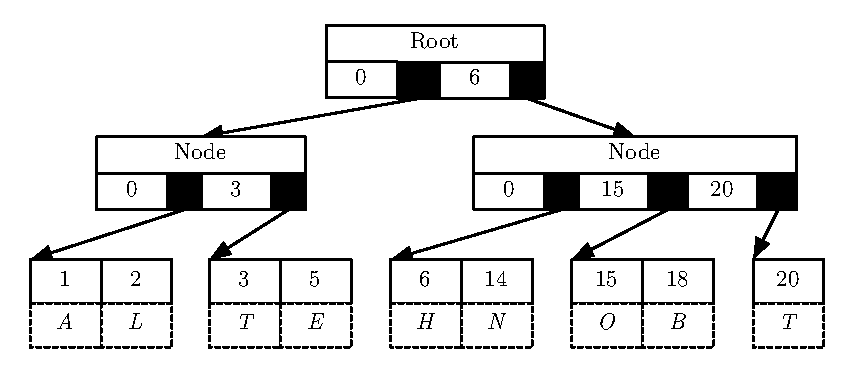
\includegraphics[width=90mm]{diagrams/BPlusTreeImpl.pdf}
 \caption{The same B+ tree as in Figure \ref{fig:bplustree} but with our specific list implementation.}
 \label{fig:bplustreeImpl}
\end{figure}

Figure \ref{fig:bplustree} correctly shows that for each node with $n$ keys there are $n+1$ pointers to sub trees. As it can be seen from both Figure \ref{fig:inductive_data_type} and \ref{fig:bplustreeImpl} we have chosen to deal with this asymmetry by always having a $0$ key in the beginning of each key-pointer list such that every node has $n+1$ key-pointer paris. Another way to represent a node would be to have $n$ key-pointer pairs as well as a start pointer of the type \begin{coqdoccode}\coqdocvar{bplustree} \coqdocvar{b} \coqdocvar{X}\end{coqdoccode}. However, that would give us unnecessary complexity both when writing our primary functions but also when proving theorems about these functions. Even though it is more strongly typed with such a definition we would always have to take care of a start pointer corner case when proving anything about our B+ trees. With our current solution we add a couple of assumptions to our notion of what a valid B+ tree is, to ensure the start pointer is properly handled. This will be explained in the following section. \todo{insert ref}

\todo{Pointers are not actually pointers - but a regular instance of a bplustree as a value}

\subsection{Valid B+ tree}
\label{subsec:Valid_bplustree}
Although this data type can represent a B+ tree, it says nothing about the validity of a tree. To make statements about a B+ tree's validity, we need a proposition that states what must hold for a B+ tree to be valid. This proposition is called $valid\_bplustree$, and can be seen in Figure \ref{fig:inductive_valid_bplustree}.

\begin{figure}
\centering
\begin{coqdoccode}
\coqdockw{Inductive} \coqdocvar{valid\_bplustree} (\coqdocvar{b}: \coqdocvar{nat}) (\coqdocvar{X}: \coqdockw{Type}) : \coqdocvar{bplustree} \coqdocvar{b} \coqdocvar{X} \ensuremath{\rightarrow} \coqdockw{Prop} :=\coqdoceol
\coqdocindent{1.00em}
\ensuremath{|} \coqdocvar{root\_is\_a\_leaf}  : \coqdockw{\ensuremath{\forall}} (\coqdocvar{kvl}: \coqdocvar{list} (\coqdocvar{nat} \ensuremath{\times} \coqdocvar{X})), \coqdoceol
\coqdocindent{11.00em}
\coqdocvar{b} \ensuremath{\not=} 0 \ensuremath{\rightarrow}\coqdoceol
\coqdocindent{11.00em}
\coqdocvar{length} \coqdocvar{kvl} \ensuremath{\le} \coqdocvar{b} \ensuremath{\times} 2 \ensuremath{\rightarrow}\coqdoceol
\coqdocindent{11.00em}
\coqdocvar{kvl\_sorted} \coqdocvar{kvl} \ensuremath{\rightarrow}  \coqdoceol
\coqdocindent{11.00em}
\coqdocvar{valid\_bplustree} \coqdocvar{b} \coqdocvar{X} (\coqdocvar{bptLeaf} \coqdocvar{b} \coqdocvar{X} \coqdocvar{kvl})\coqdoceol
\coqdocindent{1.00em}
\ensuremath{|} \coqdocvar{valid\_root\_node} : \coqdockw{\ensuremath{\forall}} (\coqdocvar{kpl}: \coqdocvar{list} (\coqdocvar{nat} \ensuremath{\times} \coqdocvar{bplustree} \coqdocvar{b} \coqdocvar{X})),\coqdoceol
\coqdocindent{11.00em}
\coqdocvar{b} \ensuremath{\not=} 0 \ensuremath{\rightarrow} \coqdoceol
\coqdocindent{11.00em}
2 \ensuremath{\le} \coqdocvar{length} \coqdocvar{kpl} \ensuremath{\rightarrow} \coqdoceol
\coqdocindent{11.00em}
\coqdocvar{length} \coqdocvar{kpl} \ensuremath{\le} \coqdocvar{S} (\coqdocvar{b} \ensuremath{\times} 2) \ensuremath{\rightarrow}\coqdoceol
\coqdocindent{11.00em}
\coqdocvar{key\_at\_index} 0 \coqdocvar{kpl} = \coqdocvar{Some} 0 \ensuremath{\rightarrow} \coqdoceol
\coqdocindent{11.00em}
\coqdocvar{all\_values} (\coqdocvar{bplustree} \coqdocvar{b} \coqdocvar{X}) (\coqdocvar{valid\_sub\_bplustree} \coqdocvar{b} \coqdocvar{X}) \coqdocvar{kpl} \ensuremath{\rightarrow}\coqdoceol
\coqdocindent{11.00em}
\coqdocvar{all\_values\_eq\_prop} (\coqdocvar{bplustree} \coqdocvar{b} \coqdocvar{X}) \coqdocvar{equal\_height} \coqdocvar{kpl} \ensuremath{\rightarrow}\coqdoceol
\coqdocindent{11.00em}
\coqdocvar{kvl\_sorted} \coqdocvar{kpl} \ensuremath{\rightarrow}  \coqdoceol
\coqdocindent{11.00em}
\coqdocvar{valid\_splits} \coqdocvar{b} \coqdocvar{X} \coqdocvar{kpl} \ensuremath{\rightarrow}\coqdoceol
\coqdocindent{11.00em}
\coqdocvar{valid\_bplustree} \coqdocvar{b} \coqdocvar{X} (\coqdocvar{bptNode} \coqdocvar{b} \coqdocvar{X} \coqdocvar{kpl})   \coqdoceol
\end{coqdoccode}
\caption{Inductive data type for a valid B+ tree.}
\label{fig:inductive_valid_bplustree}
\end{figure}

This proposition is only valid when examining the root of a tree, as there are different constraints for subtrees (See Section \ref{subsec:Background_Bplus_tree}). $valid\_bplustree$ has two cases, the first holds when the root of the B+ tree is a leaf, and the second holds when the root is a node. The various properties that must hold are explained below.

\paragraph{Root is a leaf}
The following must hold for a root leaf to be a valid B+ tree:
\label{valid_root_is_a_leaf}
\begin{itemize}
\item $b \neq 0$ --- The branching must not be 0. Since we are working with natural numbers, this means $b > 0$.
\item $length\ kvl \leq b \times 2 $ --- The leaf must have at most $2b$ elements.
\item $kvl\_sorted\ kvl$ --- The keys in the leaf must be sorted.
\end{itemize}

\paragraph{Root is a node}
The following must hold for a root node to be a valid B+ tree:
\label{valid_root_is_a_node}
\begin{itemize}
\item $b \neq 0$ --- The branching must not be 0.
\item $2 \leq length\ kpl$ and $length\ kpl \leq S\ (b \times 2)$ --- These satisfy the conditions for branching stated in Section \ref{subsec:Background_Bplus_tree}.
\item $key\_at\_index\ 0\ kpl = Some\ 0$ --- As mentioned above, we must know that the first key is always 0. This assures that this is the case.
\item $all\_values (bplustree\ b\ X)\ (valid\_sub\_bplustree\ b\ X)\ kpl$ --- All the values stored in the node (the pointers) must be valid subtrees. As mentioned in Section \ref{subsec:Background_Bplus_tree}, the constraints for the root are slightly different. The constraints for internal leaves and nodes will be covered below.
\item $all\_values\_eq\_prop (bplustree\ b\ X)\ equal\_height\ kpl$ --- All subtrees must have the same height.
\item $kvl\_sorted\ kpl$ --- The keys in the node must be sorted.
\item $valid\_splits\ b \ X\ kpl$ --- All the splits are correct, i.e. all the keys in a subtree are between the keys of its siblings.
\end{itemize}

\paragraph{}
Since $valid\_bplustree$ only holds for the root leaf or node, a different proposition is needed for internal leaves and nodes, or subtrees. This is implemented in the $valid\_sub\_bplustree$ proposition. In the interest of brevity, only the differences will be listed here:

\paragraph{Internal leaf}
\todo{Shouldn't be called internal leaf as leafs are never internal.}
\begin{itemize}
\item $b \leq length\ kvl$ --- The number of key-value pairs in the leaf must be at least $b$.
\end{itemize}

\paragraph{Internal node}
\begin{itemize}
\item $2 \leq length\ kpl$ changed to $S\ b \leq length\ kpl$ --- The number of key-pointer pairs must be at least $b+1$.
\end{itemize}

\todo{Needs some binding text before we go on with implementation.}

\subsection{Search}
\label{subsec:search}
Our implementation of search does not stray far from the prototypical version described in the background (Section \ref{sec:Background}). It is implemented through 3 functions: $search'$, $find\_subtree$, and $search\_leaf$. 
\todo{Write about sorted}

\paragraph{}
Both our $insert$ and $search$ are recursive function recursing over a descending parameter $counter$. The reason for introducing this parameter is to serve as a recursion terminator. Because our inductive type for B+ trees consists of a nesting of two inductive datatypes that are not mutually recursive, Coq is unable to reason about instances of $bplustree$ has a recursively decreasing argument. Since a key requirement for recursive Coq functions is that they must contain a decreasing argument, we introduced this notion of a counter that we will decrease by one every time we decent one down to a subtree. If the counter ever reaches $0$, the recursion stops. This means that should the counter ever reach $0$ before we have descended all the way down the tree, a wrong result will be given. To ensure this never happens, we always initialize the counter to the height of the tree.

The reason why initializing the counter to the height of the tree will guarantee that our counter will never reach $0$ before our $insert'$ implementation have descended all the way down to a leaf is simple. Our implementation of $height$ simply counts the number of steps it takes to descend down the leftmost child in every node until it reaches a leaf. Our $valid\_bplustree$ proposition captures the balancing nature of B+trees so if $height$ is called on such a valid B+ tree, the returned valid is the number of steps from the root to any leaf in the tree. So irregardless of which leaf the insert must happen in, we know we can decend that far down the tree in $counter$ steps. Because our implementation of $insert'$ only decreases the counter by one every time it recursively call itself with a subtree, we have a invariant where the counter will always be exactly equal to the height of the tree it currently processing. This invariant is a key aspect to constructing induction proofs on our B+ trees with our implementation doesn't have a datatype that is not inductively defined over the height of the tree.

\paragraph{}
A key part of both insertion and searching in our implementation is the function $find\_subtree$. This function, when given a list of key-pointer pair, and a search-key, will identify the key-pointer pair whose range contains the search-key. The pointer in the identified key-pointer pair is the subtree that, in a valid B+ tree, must contain the search-key if the tree contains the key.

\paragraph{}
The main function that performs search is $search'$, that as mentioned above is recursively defined over a natural number counter. It uses $find\_subtree$ to identify which subtree to recurse into, and when it reaches a leaf it calls $search\_leaf$. $search\_leaf$ performs a simple linear search through the key-value pairs to identify if the search-key exists within the tree.

To ensure that the counter is always initialized to the height of the tree to search, we have added a definition of $search$ that simply calls $search'$ with the $counter = height(tree)$.

\subsection{Insert}
The $insert$ function calls the $insert'$ function to insert into a tree. First $insert'$ recurses down through $counter$ layers to find the insertion point, after which it handles overflow, if any should occur, on the way back up through the recursion layers. The function $insert'$ never increases the height of the tree but lets $insert$ handle the case where the root node overflows. In this case $insert$ will split the former root node into two sub nodes and connect these to a new root. This case obviously increases the height of the tree by $1$ and keeps the tree balanced. Effectively, this means the invariant described in Section \ref{subsec:search} still holds for $insert'$, as the height of the balanced tree is always equal to the $counter$ variable, which the $insert'$ function is decreasing on.
\paragraph{}
Out of the three central $insert$, $insert'$ and $insert\_leaf$ functions the significant is $insert'$. It uses $find\_subtree$ to figure out which subtree it should recurse into and $insert\_node$ to handle overflowing subtrees. Where $insert'$ handles overflowing leafs, $insert\_node$ takes care of overflowing (non-root) nodes.

\todo{insert this somewhere else: Since Gallina does not support arrays, the only way to get lookups faster than $O(n)$ is through a tree structure, such as a B+ tree. This would add a large degree of complexity to our proofs, and since running time is not an objective of this project, it has been deemed out of scope.}

\paragraph{}
\subsection{Limitations}
\todo{Fill in...}

\subsection{Elements of a Complete Proof of Correctness}
\todo{Needs a section on what we means when we say that insert and search works}